\documentclass[usenames,dvipsnames]{beamer}
\usepackage{../../shared/styles/custom}
\usepackage{../../shared/styles/conventions}

\usepackage{color, colortbl}
\usepackage{tikz}
\usetikzlibrary{shapes.geometric, arrows, positioning, calc, trees}
\usepackage{array}
\usepackage{multirow}
\usepackage{booktabs}

% Define custom colors
\definecolor{lightblue}{RGB}{173,216,230}
\definecolor{lightgreen}{RGB}{144,238,144}
\definecolor{lightyellow}{RGB}{255,255,224}
\definecolor{lightpink}{RGB}{255,182,193}

\title{Next Token Generation}
\date{\today}
\author{Nipun Batra}
\institute{IIT Gandhinagar}

\begin{document}
\maketitle

\begin{frame}{Inspiration and Relevance}
\begin{center}
\textbf{Inspired by the great lecture from Andrej Karpathy}
\end{center}

\vspace{0.5cm}

\begin{itemize}
\item Search for "Neural Networks: Zero to Hero" to find the original lecture
\pause
\item This approach is fundamental to modern language models
\pause 
\item \textbf{Direct connection to ChatGPT:}
  \begin{itemize}
  \item Same core principle: predict the next token
  \item Scaled up from characters to words/subwords
  \item Uses transformer architecture instead of MLP
  \end{itemize}
\end{itemize}

\vspace{0.5cm}
\begin{center}
\textbf{Understanding this simple version helps grasp ChatGPT's foundation!}
\end{center}
\end{frame}

\begin{frame}{What is the Next Character?}
\begin{center}

\begin{tikzpicture}[scale=2]
% Draw the string "app"
\node[draw, rectangle, thick, minimum width=3cm, minimum height=1cm, fill=lightblue!20] at (0,0) {
\Huge \textbf{app}
};

% Question mark
\node at (2.5, 0) {\Huge \textbf{?}};
\end{tikzpicture}
\end{center}

\vspace{1cm}
\begin{center}
\textbf{\Large What is the next character?}
\end{center}
\end{frame}

\begin{frame}{Classification Task}
\begin{center}

\begin{tikzpicture}[scale=2]
% Previous string "app"
\node[draw, rectangle, thick, minimum width=3cm, minimum height=1cm, fill=lightblue!20] at (0,0) {
\Huge \textbf{app}
};

% Question mark
\node at (2.5, 0) {\Huge \textbf{?}};
\end{tikzpicture}
\end{center}

\vspace{0.5cm}
\begin{center}
\textbf{\Large We can pose this as a classification task}
\end{center}

\vspace{0.5cm}
\begin{columns}
\begin{column}{0.3\textwidth}
\begin{center}
\textbf{Input:}\\
\Large app
\end{center}
\end{column}
\begin{column}{0.7\textwidth}
\begin{center}
\textbf{Output: Probability Distribution}
\small
\begin{tabular}{|c|c||c|c|}
\hline
\textbf{Char} & \textbf{Prob} & \textbf{Char} & \textbf{Prob} \\
\hline
a & 0.01 & n & 0.01 \\
b & 0.01 & o & 0.01 \\
c & 0.01 & p & 0.01 \\
... & ... & ... & ... \\
l & \textcolor{red}{\textbf{0.45}} & z & 0.01 \\
m & 0.01 & - & 0.05 \\
\hline
\end{tabular}
\end{center}
\end{column}
\end{columns}
\end{frame}

\begin{frame}{Generate Indian Names}
\begin{center}
\textbf{Specific Problem: Generate Indian Names}
\end{center}

\vspace{0.5cm}
\begin{center}
\textbf{Dataset:}
\end{center}

\begin{columns}
\begin{column}{0.5\textwidth}
\begin{center}
\begin{tabular}{l}
Abid \\
Abhidha \\
Adesh \\
Aditya \\
Agam \\
... \\
\vdots \\
Yash \\
Yogesh \\
Zara
\end{tabular}
\end{center}
\end{column}
\begin{column}{0.5\textwidth}
\begin{itemize}
\item Collection of Indian names
\item Each name represents a sequence
\item Goal: Learn to generate similar names
\end{itemize}
\end{column}
\end{columns}
\end{frame}

\begin{frame}{Assumptions}
\begin{center}
\textbf{We'll make a few assumptions:}
\end{center}

\vspace{1cm}

\begin{enumerate}
\item \textbf{Character set:} Only use 26 lowercase characters (a-z)
\pause
\item \textbf{End marker:} A hyphen (-) indicates the end character  
\pause
\item \textbf{Length constraint:} Names are between 4 and 10 characters
\end{enumerate}

\vspace{1cm}
\begin{center}
\textbf{Total vocabulary size: 26 + 1 = 27 characters}
\end{center}
\end{frame}

\begin{frame}{Generate Training Dataset}
\begin{center}
\textbf{Creating Training Data from "abid"}
\end{center}

\vspace{0.5cm}
\begin{center}
\textbf{Using history/context of 3 characters:}
\end{center}

\vspace{0.5cm}
\begin{center}
\begin{tabular}{|c|c|c|}
\hline
\textbf{X (Input)} & & \textbf{Y (Target)} \\
\hline
[-, -, -] & $\rightarrow$ & a \\
[-, -, a] & $\rightarrow$ & b \\
[-, a, b] & $\rightarrow$ & i \\
[a, b, i] & $\rightarrow$ & d \\
[b, i, d] & $\rightarrow$ & - \\
\hline
\end{tabular}
\end{center}

\vspace{0.5cm}
\begin{center}
\textbf{Result: 5 training examples from one name "abid"}
\end{center}
\end{frame}

\begin{frame}{Representation Learning}
\begin{center}
\textbf{Important Idea: Representation Learning}
\end{center}

\vspace{0.5cm}
\begin{itemize}
\item Learn a vector representation for each character
\item Hope that similar characters will be closer in vector space
\end{itemize}

\vspace{0.5cm}
\begin{center}
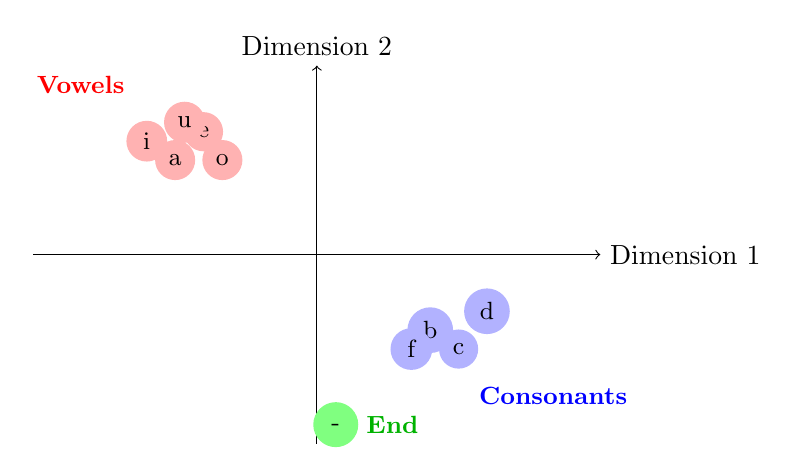
\begin{tikzpicture}[scale=1.2]
% Axes
\draw[->] (-3,0) -- (3,0) node[right] {Dimension 1};
\draw[->] (0,-2) -- (0,2) node[above] {Dimension 2};

% Vowels cluster
\node[circle, fill=red!30, inner sep=3pt] at (-1.5, 1.0) {\small a};
\node[circle, fill=red!30, inner sep=3pt] at (-1.2, 1.3) {\small e};
\node[circle, fill=red!30, inner sep=3pt] at (-1.8, 1.2) {\small i};
\node[circle, fill=red!30, inner sep=3pt] at (-1.0, 1.0) {\small o};
\node[circle, fill=red!30, inner sep=3pt] at (-1.4, 1.4) {\small u};

% Consonants cluster
\node[circle, fill=blue!30, inner sep=3pt] at (1.2, -0.8) {\small b};
\node[circle, fill=blue!30, inner sep=3pt] at (1.5, -1.0) {\small c};
\node[circle, fill=blue!30, inner sep=3pt] at (1.8, -0.6) {\small d};
\node[circle, fill=blue!30, inner sep=3pt] at (1.0, -1.0) {\small f};

% Special character
\node[circle, fill=green!50, inner sep=4pt] at (0.2, -1.8) {\small -};

% Labels
\node[color=red, font=\small\bfseries] at (-2.5, 1.8) {Vowels};
\node[color=blue, font=\small\bfseries] at (2.5, -1.5) {Consonants};
\node[color=green!70!black, font=\small\bfseries] at (0.8, -1.8) {End};
\end{tikzpicture}
\end{center}
\end{frame}

\begin{frame}{Word2Vec Reference}
\begin{center}
\textbf{Classic Word2Vec Relationship}
\end{center}

\vspace{0.5cm}
\begin{center}
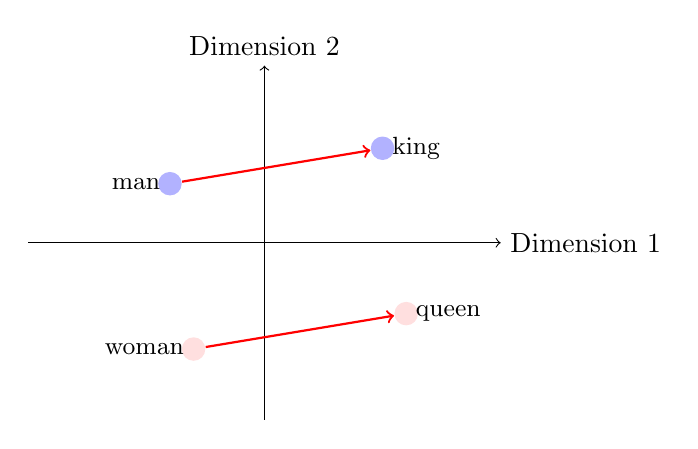
\begin{tikzpicture}[scale=1.5]
% Vector space
\draw[->] (-2,0) -- (2,0) node[right] {Dimension 1};
\draw[->] (0,-1.5) -- (0,1.5) node[above] {Dimension 2};

% Points
\node[circle, fill=blue!30, inner sep=3pt] (king) at (1, 0.8) {};
\node[right] at (king) {\small king};

\node[circle, fill=pink!50, inner sep=3pt] (queen) at (1.2, -0.6) {};
\node[right] at (queen) {\small queen};

\node[circle, fill=blue!30, inner sep=3pt] (man) at (-0.8, 0.5) {};
\node[left] at (man) {\small man};

\node[circle, fill=pink!50, inner sep=3pt] (woman) at (-0.6, -0.9) {};
\node[left] at (woman) {\small woman};

% Arrows
\draw[->, thick, red] (man) -- (king);
\draw[->, thick, red] (woman) -- (queen);
\end{tikzpicture}
\end{center}

\vspace{0.5cm}
\begin{center}
\textbf{Relationship:} queen $\approx$ king - man + woman
\end{center}
\end{frame}

\begin{frame}{Analogy with Smileys}
\begin{center}
\textbf{Emotional Expression Analogy}
\end{center}

\vspace{0.5cm}
\begin{center}
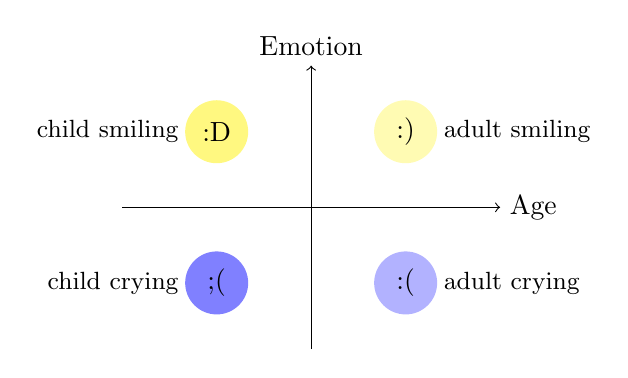
\begin{tikzpicture}[scale=1.2]
% Vector space
\draw[->] (-2,0) -- (2,0) node[right] {Age};
\draw[->] (0,-1.5) -- (0,1.5) node[above] {Emotion};

% Emotional representations using circles with symbols
\node[circle, fill=yellow!30, minimum size=0.8cm] at (1, 0.8) {:)};
\node[right] at (1.3, 0.8) {\small adult smiling};

\node[circle, fill=blue!30, minimum size=0.8cm] at (1, -0.8) {:(};
\node[right] at (1.3, -0.8) {\small adult crying};

\node[circle, fill=yellow!50, minimum size=0.8cm] at (-1, 0.8) {:D};
\node[left] at (-1.3, 0.8) {\small child smiling};

\node[circle, fill=blue!50, minimum size=0.8cm] at (-1, -0.8) {;(};
\node[left] at (-1.3, -0.8) {\small child crying};
\end{tikzpicture}
\end{center}

\vspace{0.5cm}
\begin{center}
\textbf{Relationship:} child crying = child smiling + adult crying - adult smiling
\end{center}
\end{frame}

\begin{frame}{Embedding Matrix/Table}
\begin{center}
\textbf{Main Idea: Embedding Matrix/Table}
\end{center}

\vspace{0.5cm}
\begin{center}
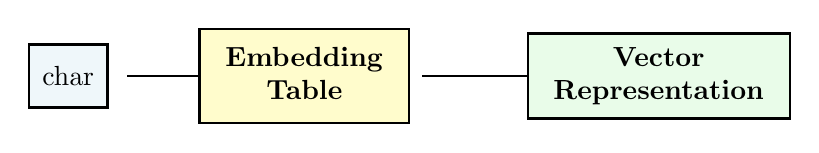
\begin{tikzpicture}[scale=1.5]
% Input character
\node[draw, rectangle, thick, minimum width=1cm, minimum height=0.8cm, fill=lightblue!20] at (-2,0) {char};

% Arrow
\draw[->, thick] (-1.5, 0) -- (-0.5, 0);

% Embedding block
\node[draw, rectangle, thick, minimum width=2cm, minimum height=1.2cm, fill=yellow!20] at (0,0) {
\begin{tabular}{c}
\textbf{Embedding} \\
\textbf{Table}
\end{tabular}
};

% Arrow
\draw[->, thick] (1, 0) -- (2, 0);

% Output vector
\node[draw, rectangle, thick, minimum width=1.5cm, minimum height=0.8cm, fill=lightgreen!20] at (3,0) {
\begin{tabular}{c}
\textbf{Vector} \\
\textbf{Representation}
\end{tabular}
};
\end{tikzpicture}
\end{center}

\vspace{0.5cm}
\begin{center}
\textbf{Process:} Character $\rightarrow$ Lookup in Embedding Table $\rightarrow$ Dense Vector
\end{center}
\end{frame}

\begin{frame}{27 × K Embedding Matrix}
\begin{center}
\textbf{Embedding Table Structure}
\end{center}

\vspace{0.3cm}
\begin{center}
\begin{tabular}{|c|c|c|c|c|}
\hline
\textbf{Char} & \textbf{D1} & \textbf{D2} & \textbf{...} & \textbf{DK} \\
\hline
a & 0.2 & -0.1 & ... & 0.8 \\
b & -0.3 & 0.5 & ... & -0.2 \\
c & 0.1 & 0.3 & ... & 0.4 \\
$\vdots$ & $\vdots$ & $\vdots$ & $\ddots$ & $\vdots$ \\
z & 0.7 & -0.4 & ... & 0.1 \\
- & 0.0 & 0.9 & ... & -0.5 \\
\hline
\end{tabular}
\end{center}

\vspace{0.5cm}
\begin{center}
\textbf{This overall becomes a 27 × K dimensional matrix}
\end{center}
\end{frame}

\begin{frame}{Learnable Matrix}
\begin{center}
\textbf{This matrix is learnable!}
\end{center}

\vspace{1cm}
\begin{itemize}
\item \textbf{Initially:} Random values
\pause
\item \textbf{During training:} Updated via backpropagation
\pause
\item \textbf{After training:} Contains meaningful character representations
\pause
\item \textbf{Similar characters:} Will have similar embedding vectors
\end{itemize}

\vspace{1cm}
\begin{center}
\textbf{The network learns both the embeddings AND the classification weights!}
\end{center}
\end{frame}

\begin{frame}{Overall Architecture (2D Example)}
\begin{center}
\textbf{Example with X = "abi" and 2D embeddings}
\end{center}

\vspace{0.3cm}
\begin{center}
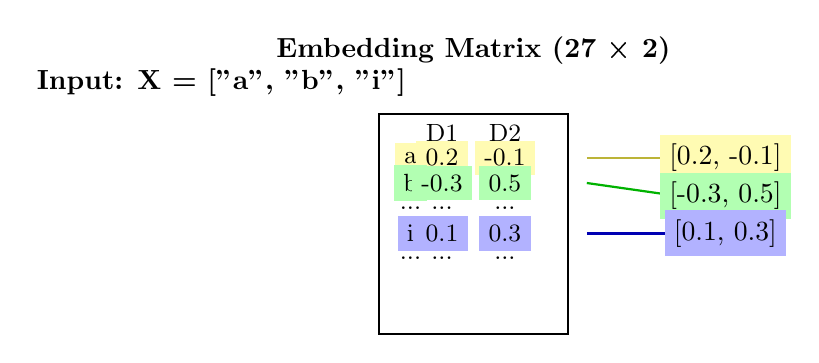
\begin{tikzpicture}[scale=0.8]
% Input vector
\node at (-4, 3) {\textbf{Input: X = ["a", "b", "i"]}};

% Embedding matrix
\node at (0, 3.5) {\textbf{Embedding Matrix (27 × 2)}};
\begin{scope}[shift={(0,0)}]
\draw[thick] (-1.5, 2.5) rectangle (1.5, -1);

% Headers
\node at (-0.5, 2.2) {\small D1};
\node at (0.5, 2.2) {\small D2};

% Character rows with colors
\node[fill=yellow!30] at (-1, 1.8) {\small a};
\node[fill=yellow!30] at (-0.5, 1.8) {\small 0.2};
\node[fill=yellow!30] at (0.5, 1.8) {\small -0.1};

\node[fill=green!30] at (-1, 1.4) {\small b};
\node[fill=green!30] at (-0.5, 1.4) {\small -0.3};
\node[fill=green!30] at (0.5, 1.4) {\small 0.5};

% Dots
\node at (-1, 1.0) {\small ...};
\node at (-0.5, 1.0) {\small ...};
\node at (0.5, 1.0) {\small ...};

\node[fill=blue!30] at (-1, 0.6) {\small i};
\node[fill=blue!30] at (-0.5, 0.6) {\small 0.1};
\node[fill=blue!30] at (0.5, 0.6) {\small 0.3};

% More dots
\node at (-1, 0.2) {\small ...};
\node at (-0.5, 0.2) {\small ...};
\node at (0.5, 0.2) {\small ...};
\end{scope}

% Arrows and extracted vectors
\draw[->, thick, yellow!70!black] (1.8, 1.8) -- (3.2, 1.8);
\node[fill=yellow!30] at (4, 1.8) {[0.2, -0.1]};

\draw[->, thick, green!70!black] (1.8, 1.4) -- (3.2, 1.2);
\node[fill=green!30] at (4, 1.2) {[-0.3, 0.5]};

\draw[->, thick, blue!70!black] (1.8, 0.6) -- (3.2, 0.6);
\node[fill=blue!30] at (4, 0.6) {[0.1, 0.3]};
\end{tikzpicture}
\end{center}
\end{frame}

\begin{frame}{Concatenate the Embeddings}
\begin{center}
\textbf{Feature Vector Creation for X = "abi"}
\end{center}

\vspace{0.5cm}
\begin{center}
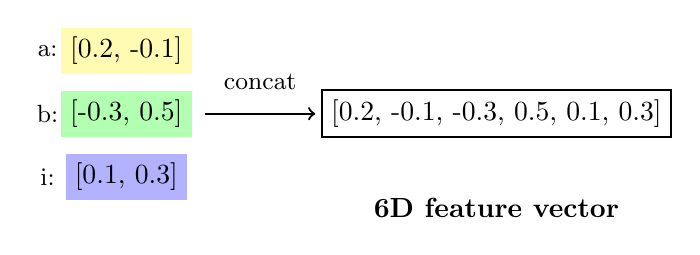
\begin{tikzpicture}[scale=1.0]
% Input embeddings
\node[fill=yellow!30, minimum width=1.3cm, minimum height=0.5cm] at (-2.2, 0.8) {[0.2, -0.1]};
\node at (-3.2, 0.8) {\small a:};

\node[fill=green!30, minimum width=1.3cm, minimum height=0.5cm] at (-2.2, 0) {[-0.3, 0.5]};
\node at (-3.2, 0) {\small b:};

\node[fill=blue!30, minimum width=1.3cm, minimum height=0.5cm] at (-2.2, -0.8) {[0.1, 0.3]};
\node at (-3.2, -0.8) {\small i:};

% Arrow
\draw[->, thick] (-1.2, 0) -- (0.2, 0);
\node at (-0.5, 0.4) {\small concat};

% Result
\node[draw, rectangle, thick, minimum width=3.5cm, minimum height=0.6cm] at (2.5, 0) {
[0.2, -0.1, -0.3, 0.5, 0.1, 0.3]
};

\node at (2.5, -1.2) {\textbf{6D feature vector}};
\end{tikzpicture}
\end{center}

\vspace{0.3cm}
\begin{center}
\textbf{The feature vector pulls up embeddings and concatenates them}
\end{center}
\end{frame}

\begin{frame}{Multi-Layer Perceptron}
\begin{center}
\textbf{Neural Architecture}
\end{center}

\vspace{0.5cm}
\begin{center}
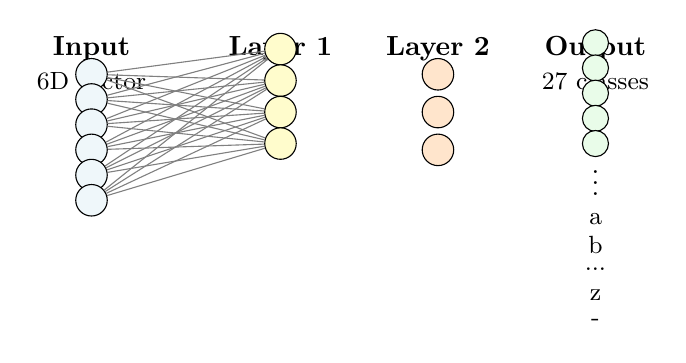
\begin{tikzpicture}[scale=0.8]
% Input layer
\node at (-4, 3) {\textbf{Input}};
\node at (-4, 2.5) {\small 6D vector};
\foreach \i in {1,2,3,4,5,6} {
    \node[circle, draw, fill=lightblue!20, minimum size=0.4cm] (input\i) at (-4, 3-\i*0.4) {};
}

% Hidden layer 1
\node at (-1, 3) {\textbf{Layer 1}};
\foreach \i in {1,2,3,4} {
    \node[circle, draw, fill=yellow!20, minimum size=0.4cm] (hidden1\i) at (-1, 3.5-\i*0.5) {};
}

% Hidden layer 2
\node at (1.5, 3) {\textbf{Layer 2}};
\foreach \i in {1,2,3} {
    \node[circle, draw, fill=orange!20, minimum size=0.4cm] (hidden2\i) at (1.5, 3.2-\i*0.6) {};
}

% Output layer
\node at (4, 3) {\textbf{Output}};
\node at (4, 2.5) {\small 27 classes};
\foreach \i in {1,2,3,4,5} {
    \node[circle, draw, fill=lightgreen!20, minimum size=0.3cm] (output\i) at (4, 3.5-\i*0.4) {};
}
\node at (4, 1) {\vdots};

% Sample connections
\foreach \i in {1,2,3,4,5,6} {
    \foreach \j in {1,2,3,4} {
        \draw[gray, thin] (input\i) -- (hidden1\j);
    }
}

% Labels
\node at (4, 0.3) {\small a};
\node at (4, -0.1) {\small b};
\node at (4, -0.5) {\small ...};
\node at (4, -0.9) {\small z};
\node at (4, -1.3) {\small -};
\end{tikzpicture}
\end{center}

\vspace{0.3cm}
\begin{center}
\textbf{Eventually shows 27-class output vector}
\end{center}
\end{frame}

\begin{frame}{Cross-Entropy Loss}
\begin{center}
\textbf{Learning Process}
\end{center}

\vspace{0.5cm}
\begin{itemize}
\item \textbf{Loss Function:} Use cross-entropy loss to learn
\pause
\item \textbf{We are learning two things:}
  \begin{enumerate}
  \item The embedding matrix (27 × K parameters)
  \item The MLP weights (neural network parameters)
  \end{enumerate}
\pause
\item \textbf{Training Process:}
  \begin{itemize}
  \item Forward pass: Input → Embeddings → Concatenate → MLP → Probabilities
  \item Compute cross-entropy loss against true next character
  \item Backward pass: Update both embeddings and MLP weights
  \end{itemize}
\end{itemize}
\end{frame}

\begin{frame}{Generate/Sample from Learned Model}
\begin{center}
\textbf{Test Input: "abi"}
\end{center}

\vspace{0.5cm}
\begin{center}
\textbf{Probability vector for next character:}
\end{center}

\vspace{0.3cm}
\begin{center}
\begin{tabular}{|c|c||c|c|}
\hline
\textbf{Next Char} & \textbf{Probability} & \textbf{Next Char} & \textbf{Probability} \\
\hline
a & 0.01 & n & 0.05 \\
b & 0.01 & o & 0.02 \\
c & 0.03 & p & 0.01 \\
d & \textcolor{red}{\textbf{0.60}} & ... & ... \\
... & ... & z & 0.01 \\
\hline
\end{tabular}
\end{center}

\vspace{0.5cm}
\begin{itemize}
\item ABIA would be 1\%
\item ABIB would be 1\%  
\item \textbf{ABID would be 60\%}
\end{itemize}
\end{frame}

\begin{frame}{Tree Structure}
\begin{center}
\textbf{Generation as Tree Structure}
\end{center}

\vspace{0.5cm}
\begin{center}
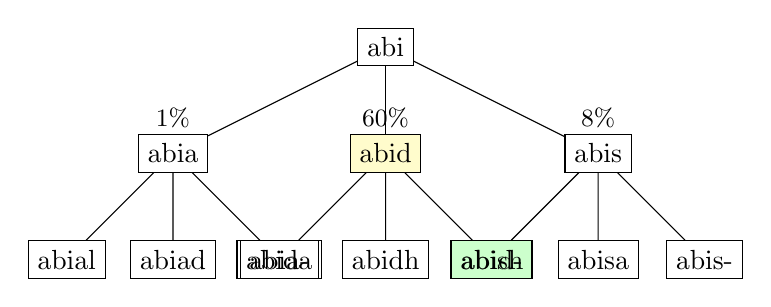
\begin{tikzpicture}[scale=0.9, level 1/.style={sibling distance=3cm}, level 2/.style={sibling distance=1.5cm}]
\node[draw, rectangle] {abi}
    child {
        node[draw, rectangle] {abia}
        child {node[draw, rectangle] {abial}}
        child {node[draw, rectangle] {abiad}}
        child {node[draw, rectangle] {abia-}}
    }
    child {
        node[draw, rectangle, fill=yellow!20] {abid}
        child {node[draw, rectangle] {abida}}
        child {node[draw, rectangle] {abidh}}
        child {node[draw, rectangle, fill=green!20] {abid-}}
    }
    child {
        node[draw, rectangle] {abis}
        child {node[draw, rectangle] {abish}}
        child {node[draw, rectangle] {abisa}}
        child {node[draw, rectangle] {abis-}}
    };

% Probabilities
\node at (-3, -1) {\small 1\%};
\node at (0, -1) {\small 60\%};
\node at (3, -1) {\small 8\%};
\end{tikzpicture}
\end{center}

\vspace{0.3cm}
\begin{center}
\textbf{Had we chosen A, it starts a new branch. Had we chosen D, it starts a new branch, etc.}
\end{center}
\end{frame}

\begin{frame}{Temperature Term}
\begin{center}
\textbf{Temperature in Softmax}
\end{center}

\vspace{0.5cm}
\begin{itemize}
\item \textbf{Standard Softmax:}
\begin{equation}
P(y_i) = \frac{e^{z_i}}{\sum_{j=1}^{27} e^{z_j}}
\end{equation}

\pause
\item \textbf{Temperature-scaled Softmax:}
\begin{equation}
P(y_i) = \frac{e^{z_i/T}}{\sum_{j=1}^{27} e^{z_j/T}}
\end{equation}

\pause
\item \textbf{Temperature Effects:}
\begin{itemize}
\item $T = 1$: Default/standard probabilities
\item $T \to 0$: Very low temperature → more peaked (deterministic)
\item $T \to \infty$: Very high temperature → more uniform (random)
\end{itemize}
\end{itemize}
\end{frame}

\begin{frame}{Temperature Variations}
\begin{center}
\textbf{How sampling differs across temperatures}
\end{center}

\vspace{0.3cm}
\begin{center}
\begin{tabular}{|c|c|c|c|}
\hline
\textbf{Next Char} & \textbf{Default} & \textbf{Low T} & \textbf{High T} \\
 & \textbf{T=1.0} & \textbf{T=0.5} & \textbf{T=2.0} \\
\hline
a & 0.01 & 0.001 & 0.08 \\
d & \textcolor{red}{\textbf{0.60}} & \textcolor{red}{\textbf{0.95}} & \textcolor{red}{\textbf{0.25}} \\
s & 0.08 & 0.01 & 0.12 \\
h & 0.03 & 0.005 & 0.09 \\
- & 0.05 & 0.02 & 0.11 \\
others & 0.23 & 0.015 & 0.35 \\
\hline
\end{tabular}
\end{center}

\vspace{0.5cm}
\begin{itemize}
\item \textbf{Low Temperature:} Conservative, predictable generation
\item \textbf{High Temperature:} Creative, diverse generation
\end{itemize}
\end{frame}

\end{document}